% Отчет по лабораторной работе №2
% Рыжиков И.С. 2022г
%=== Тип документа - статья, кегль 14пт.
\documentclass[14pt]{article}
%=== Настройка кодировок, шрифта и языка
\usepackage[utf8]{inputenc}
\usepackage{extsizes}
\usepackage[main=russian, english]{babel}
\usepackage[T2A, T1]{fontenc}
%=== Разметка документа
\usepackage{geometry} 
\geometry{
	a4paper, 
	top = 2cm,
	bottom = 2cm,
	left = 3cm,
	right = 1.5cm
}
%=== Стилизация номера страницы
\usepackage{fancyhdr}

% \pagestyle{fancy}
% \fancyhf{}
% \rfoot{\thepage}

%=== Форматирование текста
\usepackage{setspace}			% Интерлиньяж
\onehalfspacing					% 1.5 строки
\usepackage{indentfirst} 		% Красная строка с первого предложения
\setlength						% Отступ красной строки - 1.25см
	{\parindent}
	{1.25cm}	
\usepackage{titlesec}			% Форматирование заголовков
\titleformat					% Разделы
	{\section}
	[hang]
	{\normalfont\bfseries}
	{}
	{0pt}
	{}
\titlespacing
	{\section}
	{\parindent}
	{4ex}
	{0pt}
\titleformat					% Подразделы
	{\subsection}
	[hang]
	{\normalfont\itshape}
	{}
	{0pt}
	{}
\titlespacing
	{\subsection}
	{\parindent}
	{4ex}
	{0pt}

%=== Минимизируем количество переносов
\usepackage{ragged2e}
\usepackage{microtype}
\tolerance = 500
\hyphenpenalty = 20000
\emergencystretch = 1cm
%=== Таблицы
\usepackage{tabularx}	% основной тип таблиц, выравнивание по ширине
\usepackage{longtable}	% для таблиц, не вмещающихся на одну страницу
\usepackage{multirow}	% для разбиения ячеек на несколько строк
\usepackage{multicol}	% на несколько колонок
%=== ^ до этого места - минимальная преамбула документа.
%=== Далее идут опциональные, но часто использующиеся пакеты,
%=== а так же написанные мной команды, чем-то упрощающие написание отчетов
\usepackage{array}
%=== Меняем подписи к таблицам
\usepackage{caption}
\captionsetup[table]{singlelinecheck=off, justification=RaggedRight}

%=== Работа с формулами
% Набор пакетов, сильно расширяющих возможности по набору формул
\usepackage{amsmath}
% добавляет специфические для русских  статей мат. символы вроде \leqslant
\usepackage{amssymb}
% добавляет окружения для теорем и лемм	
\usepackage{amsthm}				
\usepackage{mathtools}
% номера только для тех формул, на которые есть ссылки в тексте
\mathtoolsset{showonlyrefs=true}
%=== Работа с изображениями
\usepackage{wrapfig}
\usepackage{graphicx}
\graphicspath{ {./images/} }
%=== Работа с гиперссылками
\usepackage[unicode]{hyperref}
\hypersetup{
	colorlinks=true,
	urlcolor=blue,
	filecolor=green,
	linkcolor=red
}

\begin{document}
\pagenumbering{gobble}
\clearpage
\begin{center}	
	МИНОБРНАУКИ РОССИИ\\
	САНКТ-ПЕТЕРБУРГСКИЙ ГОСУДАРСТВЕННЫЙ\\
	ЭЛЕКТРОТЕХНИЧЕСКИЙ УНИВЕРСИТЕТ\\
	«ЛЭТИ» ИМ. В.И. УЛЬЯНОВА (ЛЕНИНА)\\
    Кафедра Физики
	\vspace{54mm}

	ОТЧЕТ\\
	по лабораторной работе №2 \\
	Тема: «Исследование динамики свободных \\
    гармонических колебаний в поле силы тяжести»\\



	\vspace{65mm}

	\def\arraystretch{1.5}
	\begin{tabularx}{\textwidth}{ >{\hsize=7cm}X >{\hsize=4cm}X  >{\centering\arraybackslash}X }
		Студент гр. 2381 & & Рыжиков И.С. \\ \cline{2-2}
		Преподаватель & & Агабабаев В.А. \\ \cline{2-2}
	\end{tabularx}
	\def\arraystretch{1}

	\vfill
	Санкт-Петербург\\
	2022
\end{center}
\newpage
% \pagenumbering{arabic}
% \setcounter{page}{2}
\section{Цель работы}
Изучение закономерностей колебательного движения тела в однородном поле силы тяжести; исследование процессов превращения энергии в консервативных системах; определение момента инерции физического маятника.

\section{Приборы и принадлежности}
\begin{wrapfigure}[13]{r}{0.25\textwidth}
    \centering
    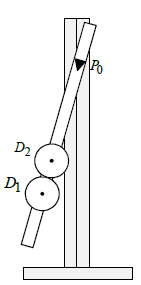
\includegraphics{маятник.png}
    \caption{}
    \label{fig:pendulum}
\end{wrapfigure}
Физический маятник; секундомер; масштабная линейка, чертежный треугольник.

Конструкция оборотного маятника представлена на рис. \ref*{fig:pendulum}. На стержне 1 закреплены два диска – D1 и D2. Маятник может быть подвешен на кронштейне к легкой
призме, трение в которой пренебрежимо мало.

\section{Исследуемые закономерности}

Физический маятник - это тело с распределенной массой или система тел, ось вращения которого расположена выше центра масс маятника. Относительно этой оси маятник колеблется с периодом
\begin{equation}\label{eq:Period}
    T_0=2 \pi \sqrt{\frac{I}{m g x_c}}=2 \pi \sqrt{\frac{l_0}{g}}
\end{equation}
где для составного маятника $m=\sum m_i$ - масса маятника, $x_c=\frac{1}{m} \sum m_i x_{c i}-$ положение его центра масс относительно оси вращения, $m_i$ и $x_{c i}-$ масса $i-$ го тела и положение его центра масс относительно оси вращения, $I=\sum I_i-$ полный момент инерции маятника, $I_i=I_{0 i}+m_i x_{c i}^2-$ момент инерции і-го тела, рассчитанный относительно оси вращения по теореме Штейнера, $I_{0 i}-$ момент инерции этого тела относительно его центра масс. Длина математического маятника, период которого совпадает с периодом колебаний данного физического маятника называется приведенной длиной физического маятника. Ее можно найти как $l_0=I / m x_c=g T_0^2 / 4 \pi^2$. Ее можно определить экспериментально, если найти новую ось $O^{\prime}$, называемую осью качания, относительно которой маятник колеблется с тем же периодом $T_0$, что и относительно оси вращения $O$. Расстояние между осями вращения и качания $O O^{\prime}=l_0$ и будет приведенной длиной физического маятника.
Полный момент инерции маятника может быть представлен в виде:
\begin{equation}\label{eq:fullMomentOfInertion}
    I=I_0+m \overline{x_c^2}
\end{equation}
где $I_0=\sum I_{0 i}, \overline{x_c^2}=\frac{1}{m} \sum m_i x_{c i}^2-$ средний квадрат положений центров масс системы тел, составляющих маятник.

Если период колебаний маятника определен экспериментально, то из
\eqref{eq:Period} можно найти момент инерции маятника:
\begin{equation}\label{eq:momentOfInertion}
    I=m g x_{\mathrm{c}} T_0^2 / 4 \pi^2 .
\end{equation}
\subsection{Сохранение энергии гармонических колебаний.}
Поскольку физический маятник, качающийся под действием силы тяжести, является консервативной системой, можно проанализировать процесс перехода потенциальной энергии маятника в кинетическую и обратно.

Потенциальная энергия при достижении амплитудного значения угла отклонения маятника равна:
\begin{equation}\label{eq:potentionEnergy}
    W_{\mathrm{pm}}=m g h_{\mathrm{c}}=m g x_{\mathrm{c}}\left(1-\cos \varphi_{\mathrm{m}}\right)=2 m g x_{\mathrm{c}} \sin ^2 \frac{\varphi_{\mathrm{m}}}{2} \approx \frac{1}{2} m g x_{\mathrm{c}} \varphi_{\mathrm{m}}^2
\end{equation}

где $h_c$ - высота поднятия центра масс маятника при его максимальном отклонении от положения равновесия, $x_{\mathrm{c}}-$ положение центра масс маятника относительно его точки подвеса, $\varphi_{\mathrm{m}}-$ максимальный угол отклонения маятника от положения равновесия.

При малых углах отклонения маятника (до $20^{\circ}$ ) максимальная потенциальная энергия равна:
\begin{equation}\label{eq:maxPotentionEnergy}
    W_{\mathrm{pm}} \approx \frac{1}{2} m g x_{\mathrm{c}} \varphi_{\mathrm{m}}^2 .
\end{equation}
Максимальная кинетическая энергия физического маятника
\begin{equation}\label{eq:maxKeneticEnergy}
    W_{\mathrm{km}}=\frac{I \omega_{\mathrm{m}}^2}{2}=\frac{m g x_{\mathrm{c}} T_0^2 \omega_{\mathrm{m}}^2}{8 \pi^2},
\end{equation}
где момент инерции маятника выражен по формуле \eqref{eq:momentOfInertion} через период его колебаний. Из закона сохранения полной механической энергии
\begin{equation}\label{eq:conservationOfEnergy}
    W=W_k+W_p=W_{\mathrm{km}}=W_{\mathrm{pm}}=\text { const }
\end{equation}
можно найти максимальную угловую скорость маятника при прохождении им положения равновесия $\omega_{\mathrm{m}}=2 \pi \varphi_{\mathrm{m}} / T_0$.

\newpage

\section{Вопросы}

9.	Напишите уравнение для кинетической и потенциальной энергии физического маятника. Найдите полную энергию. Какой характер сил, действующих на качающееся тело, консервативный или диссипативный?

Ответ:
Потенциальная энергия  равна:
\begin{equation}\label{equestionsEq:potentionEnergy}
    W_{\mathrm{p}}
    =m g h_{\mathrm{c}}
    =m g x_{\mathrm{c}}\left(1-\cos \varphi\right)
    =2 m g x_{\mathrm{c}} \sin ^2 \frac{\varphi}{2}
    \approx \frac{1}{2} m g x_{\mathrm{c}} \varphi^2
\end{equation}
где $h_c$ - высота поднятия центра масс маятника при его максимальном отклонении от положения равновесия, $x_{\mathrm{c}}$ - положение центра масс маятника относительно его точки подвеса, $\varphi$ - угол отклонения маятника от положения равновесия.

Кинетическая энергия маятника
\begin{equation}\label{equestionsEq:keneticEnergy}
    W_{\mathrm{k}}=\frac{I \omega^2}{2}
\end{equation}

На качающееся тело действуют сила тяжести и сила упругости, которые является консервативными силами.


1.	Какие силы называются консервативными?

Ответ:

Консервативные силы — силы, работа которых по замкнутой траектории равна 0.

\newpage
% \section{Основные используемые формулы}
%=== 1 задание обработки
%=== 2 задание обработки
Период колебаний маятника:
\begin{equation}\label{mainEq:period}
    T=t/n .
\end{equation}

%=== 3 задание обработки
Момент инерции маятника:
\begin{equation}\label{mainEq:momentOfInertion}
    I=m g x_{\mathrm{c}} T_0^2 / 4 \pi^2 .
\end{equation}

%=== 4 задание обработки
Полная механическая энергия маятника:
\begin{equation}\label{mainEq:potentionEnergy}
    W = W_{\mathrm{pm}} \approx \frac{1}{2} m g x_{\mathrm{c}} \varphi_{\mathrm{m}}^2 .
\end{equation}

%=== 5 задание обработки
Приведенная длина маятника:
\begin{equation}\label{eq:approxLength}
    l_0=I / m x_c=g T_0^2 / 4 \pi^2 .
\end{equation}

%=== 6 задание обработки 
%=== 7 задание обработки
Положение центра масс:

%=== 8 задание обработки
Моменты инерции каждого из тел составного маятника и его полный момент инерции $I = \sum I_i$

\newpage
\section{
    \centering
  ПРОТОКОЛ НАБЛЮДЕНИЙ \\*
  ЛАБОРАТОРНАЯ РАБОТА №1 \\*
  «Определение коэффициента трения покоя» \\
 }

\begin{table}[h!]
    \caption{}
    \label{table:protocol1}
    \begin{center}
        \begin{tabularx}{\textwidth}{ | >{\centering}X   *{5}{| >{\raggedright}X} | >{\centering}X | }
            \hline
            \      & 1 & 2 & 3 & 4 & 5 & $\theta$ \tabularnewline
            \hline
            $t, c$ &   &   &   &   &   & \        \tabularnewline [2.5ex]
            \hline
        \end{tabularx}
    \end{center}
\end{table}


\begin{table}[h!]
    \caption{}\label{table:protocol2}
    \begin{center}
        \begin{tabularx}{\textwidth}{ *2{| >{\raggedright}X} | >{\raggedright}c | >{\raggedright}c  *{7}{| >{\raggedright}X}|}
            \hline
            $l$ & $d$ & $D_1= D_2$ & $h_1=h_2$ & $m$ & $\rho$ & $x_c$ & $x_1$ & $x_2$ & $x_3$ \tabularnewline
            \hline
                &     &            &           &     &        &       &       &       & \tabularnewline [2.5ex]
            \hline
        \end{tabularx}
    \end{center}
\end{table}

\vfill

\begin{center}
    \def\arraystretch{1.5}
    \begin{tabularx}{\textwidth}{ >{\hsize=7cm}l >{\hsize=3cm}p{4cm}  >{\centering\arraybackslash}r }
        Выполнил                                                 &   \multicolumn{2}{l}{Рыжиков И.С.}   \\
                                                                 &  \multicolumn{2}{l}{Факультет КТИ}  \\
                                                                 &  \multicolumn{2}{l}{Группа № 2381}  \\
        \multicolumn{3}{l}{“\rule{1.25cm}{0.25pt}” \rule{4cm}{0.25pt} \rule{2cm}{0.25pt}}                 \\
        Преподаватель:                                           &  & Агабабаев В.А. \\ \cline{2-2}
    \end{tabularx}
    \def\arraystretch{1}
\end{center}

\newpage





% \section{Экспериментальные результаты.}
% Приводятся экспериментальные данные, в том числе результаты моделирования (обычно в виде таблиц).

% \section{Обработка результатов эксперимента.}
% Приводятся результаты обработки экспериментальных данных, результаты расчетов, графики полученных зависимостей, иные требуемые методическими указаниями данные.

% \section{Выводы.}
% Оценивается степень соответствия полученных результатов расчетов и экспериментов с теоретическими данными.

% Дается объяснение полученных в ходе работы зависимостей и результатов. \newline

% \textit{Студенты имеют право оформлять отчет как в рукописном варианте, так и использовать для оформления и печати ЭВМ и МФУ.	}

\end{document}